\chapter{자원의 평가 요소}
자원을 사용하게 되면 상대가 반응하여 자원을 소모하게 된다. 또는 상대가 자원을 사용했을 때 반응하여 자원을 사용하게 된다. 이 때 자원 사용의 결과를 예측하고 가장 좋은 결과를 낼 수 있는 방식으로 자원을 투자하려면 평가의 기준이 필요하다. 자원 사용의 결과를 평가하는 기준으로 시간과 공간, 그리고 상대의 자원이라는 세 가지 관점을 알아보자.
\section{시간 : 오버워치의 흐름이자 플레이의 기준}
오버워치에는 탄창, 체력, 스킬 등의 여러 자원이 존재하고, 이 자원들의 공통점은 사용하고 나면 다시 채워야 한다는 점이다. 채우는 데에는 시간이 필요하고, 이 시간동안 캐릭터는 약해지거나 무력해진다. 예를 들어, 구르기가 없는 맥크리는 장전에 1.2초가 걸리고, 메르시의 부활 캐스팅 시간은 1.75초이므로 탄창을 세서 부활타이밍을 잴 수 있다.
파라의 부스터 재사용 대기 시간은 8초이며 메르시가 이 시간을 생각하며 이동하면 파라를 시선에서 놓치더라도 쉽게 발견할 수 있다. 이처럼 오버워치에는 사이클이 존재하며 이 사이클마다 정보수집(Read),상황판단(Decision making),계획(Plan),실행(Do),피드백(Feedback)의 다섯 단계를 밟아나가야 한다.
오버워치의 시간 사이클은 세 가지로 구분할 수 있다.
\begin{enumerate}
    \item 10초 내외의 각 캐릭터의 사이클\label{cyc:1}\\
    이 사이클은 스킬을 사용하고 쿨타임 동안, 체력이 빠지고 다시 채울 때까지의 사이클이다. 섬광탄이 빠진 맥크리는 레킹볼-트레이서 포커싱에서 살 수 없다. 체력이 빠진 젠야타는 다시 채워지기 전까지 자리를 옮기기 어렵다. 이러한 각 영웅의 사이클이 한타의 사이클을 만드는데, 각 팀 탱커의 스킬을 기준으로
    \begin{itemize}
        \item 아군의 진입턴 : 어떻게 킬을 낼 것인가? 상대가 버티는 것을 어떻게 차단할것인가?
        \item 상대의 진입턴 : 어떻게 버틸 것인가? 잘 하면 역으로 변수를 만들 수도 있지 않을까?
    \end{itemize}
        
    이 결정된다. 라자조합에서의 자리야 방벽 및 라인하르트 방벽, 윈디조합에서의 호빵 및 매트릭스가 이에 해당한다. 여기에 나머지 영웅의 궁극기 등 자원상황을 추가적으로 고려한다. \textbf{이는 오버워치 플레이의 가장 중요한 기준이 된다.}두 턴 모두에서 주의해야 할 점은 내가 죽지 않는 것, 아군을 죽이지 않으면서 상대를 죽이는 것이다. 이 관점을 기준으로 각 포지션의 역할을 생각해보자. 아군의 진입턴에서의 각 포지션별 역할을 가볍게 생각해보자. 아군의 진입턴에서 탱커는 
    아군의 힐각과 딜각 생각하면서 진입하기. 진입의 근거 만들기. 예) 상대 방벽이 없고 우리는 있을 때, 상대 힐벤이 빠졌을 때 진입한다.
    \item 30초에서 1분 내외의 한타 준비-전개 단위 사이클\\
    이 사이클은 \nameref{cyc:1}이 여러 번 반복되는 네 단계로 이루어진다. 이 때 단계는 \nameref{cyc:1} 의 1회 수행마다 한 단계가 진행될 수도 있고, 여러 단계가 진행될 수도 있고, 궁극기 파밍 외에 아무런 소득도 없을 수도 있다.
    \begin{enumerate}
        \item pre-fighting: 대치와 한타 계획 \\
        한타 이전에는 이 다음에 벌어질 한타를 위해 자원을 모으고 한타 과정을 계획해야 한다. 특히 첫 싸움의 경우 한타 계획 단계에서 서로의 조합을 비교해야 한다.
        \begin{itemize}
            \item 조합 변경점 체크하기. 마지막 턴이고 아군이 가진 수비궁이 없지만, 상대가 중력자탄을 가지고 있다면 지원가가 바티스트, 탱커가 디바를 꺼내서 카운터를 시도할 수 있다. 상대가 조합 변경점을 인지하지 못한다면, 매트릭스에 차단당할 확률이 높을 것이다. 이와 같이, 조합의 변경점을 체크한 상태에서 플레이를 준비해야 한다.
            \item 상대가 가진 자원과 아군이 가진 자원 계산하기: 주로 궁극기를 체크하고 상대의 궁극기를 카운터할 방법과 아군의 궁극기 사용 및 효율적인 포커싱, 힐을 위한 동선과 스킬 사용 순서를 계획한다. 초심자는 "오버워치는 턴제 궁극기 교환 싸움이다."  "궁극기는 2턴마다 한번씩 돈다" "궁극기를 카운터할 수 있는 방법은 여러 가지이다" 만 우선 기억하도록 하자.
            \item궁극기 계산 요소
            \begin{enumerate}
                \item 상대의 딜량 기반으로 예측하기 예) 화염강타 한대당 10\%
                \item 아군의 힐량 기반으로 예측하기 예) 아군 힐러 궁이 빠르면 상대 딜러들의 궁이 빠름
                \item 아군의 플레이방식, 적군의 플레이방식 기반으로 예측하기 예) 겐지가 뒷라인 암살만 노릴 때보다 앞라인과 딜교환을 오래하면 용검이 20초정도 빨리찬다. 
            \end{enumerate}
            \item 아군이 가진 자원을 적절히 사용하기 위해 상대가 가진 자원을 소모시키기. ex)화강, 모이라 구슬으로 매트릭스 빼고 자탄, 자탄 쓰기 전에 상대를 한쪽으로 몰아넣기.
            \item 아군의 궁극기 및 스킬 등 자원을 채움. ex) 자리야 게이지 채운 후 방벽 쿨타임 돌리기. +상대 방벽 갈기, 매트릭스 빼기도 동시에 생각
            \item 우리 팀이 싸우기 좋은 위치로 자리를 옮기며 상대를 밀어내거나 끌어들여 한타 유도하기. ex) 용검이 있으면 뒤로 빠져서 방밀포커싱 또는 방밀수면 준비하기, 이엠피가 있으면 수비궁 가진 인원 숨어있기, 솜브라 찾아서 이엠피 이니쉬 템포 늦추기, 아군이 렐리가 있으면 앞라인 체력싸움 걸기 등
        \end{itemize}
        
        
    \end{enumerate}
    \item 포인트 단위 사이클
    \newline 아이헨발데 2거점을 예로 들어보자. 코너는 2개가 있고, 수비 입장에서 화물이 첫 코너 를 돌기 전에 오랜 시간동안 막다가 한타를 져서 그 다음 턴을 가야한다고 하자. 이 때 
\end{enumerate}

\section{공간 : 오버워치의 전장 목표}
오버워치의 전장목표는 상대의 공간을 뺏어오거나 아군의 공간을 지키는 것이다. 자원을 제대로 사용하지 못하거나 아군이 자원을 사용하면서 공간을 창출할 때 만들어진 공간을 활용하지 못하면 상대에게 공간을 내주게 된다. 주요 공간을 지키기 위해서는 자원을 사용하는 위치를 잘 생각해야 한다. 예를 들어, 윈스턴이 방벽을 상대의 힐각을 완벽히 차단하는 위치로 설치하면서, 아군의 힐각과 딜각을 고려한 위치로 점프한다면, 해당 한타는 이길 확률이 매우 높을 것이다. 하지만 윈스턴 입장에서 아군 힐러와 딜러들의 동선을 체크하면서 동시에 상대 힐러들을 압박하기는 어려우므로, 윈스턴이 점프한 직후 아군 힐러와 딜러들은 힐각과 딜각이 열리는 위치로 바로 이동해주어야 한다.\footnote{팀의 포지션은 아이돌 춤 같은 거라서, 한 명이 어그러지면 바로 상대의 진입각이 열린다.}
\section{connectivity : 공간에 대한 부연설명}
예시를 보면서 설명하겠다.\cite{rz_form}
\begin{figure}[H]
    \centering
    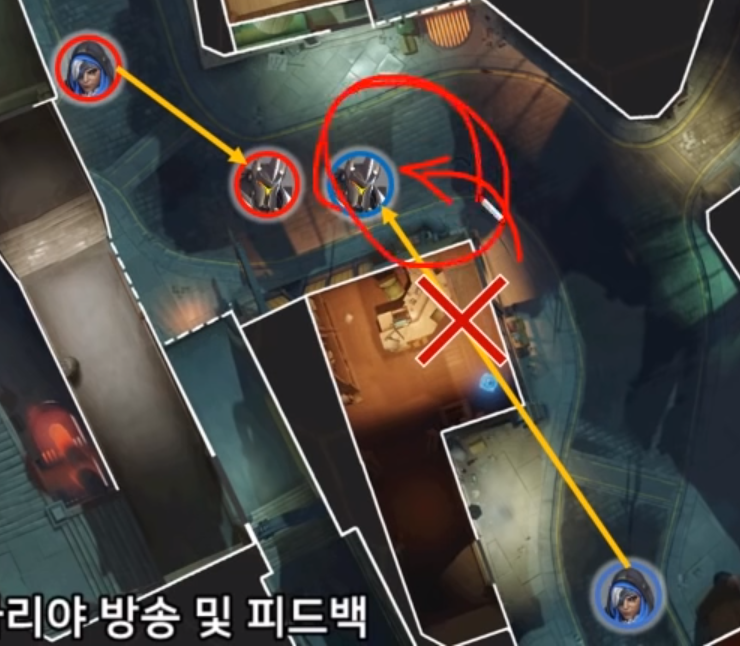
\includegraphics[width=0.6\textwidth]{figures/rz_form/disconneted.png}
    \caption{라자 포메이션 싸움 1: disconnection 발생}
    \label{fig:RZ_1}
\end{figure}
오버워치의 홀딩 위치는 좁은 길목 또는 코너이다. 이를 달리 말하면 진입하는 입장에서 앞라인과 뒷라인의 연결이 끊기는 위치이다.
\begin{figure}[H]
    \centering
    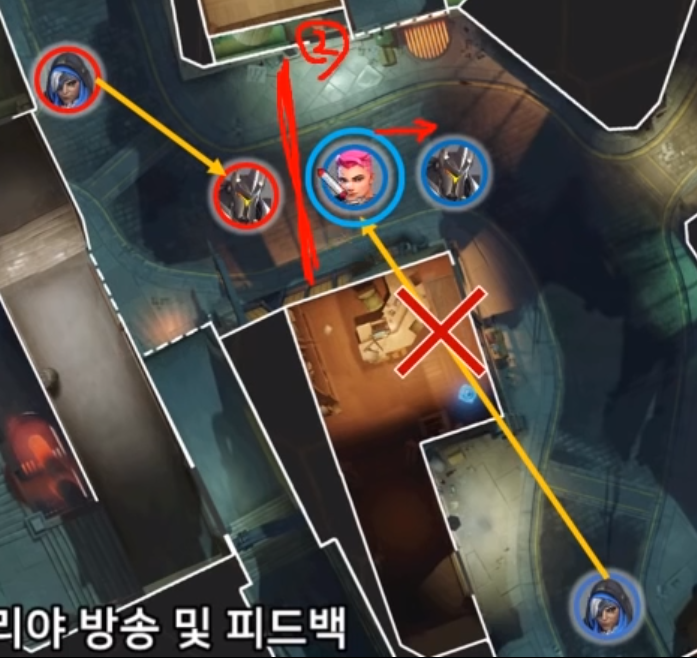
\includegraphics[width=0.6\textwidth]{figures/rz_form/bubble.png}
    \caption{라자 포메이션 싸움 2: disconnection 메꾸기}
    \label{fig:RZ_2}
\end{figure}
따라서 이 잠깐의 힐 공백을 메꾸고 및 진입시 들어오는 압박을 막기 위해 자리야가 라인하르트에게 방벽을 씌워주고, 자가 방벽으로 스스로 엄폐물이 되어 막아준다.

방벽이 모두 소모되기 전에 뒷라인이 연결되어 다시 힐할 수 있는 상태가 되어야 다음 코너까지의 공간을 수비측과 동등하게 사용할 수 있다.
그러나 수비측은 공간을 미리 장악하고 있으므로 이러한 disconnetion이 발생하지 않으며, 같은 방식으로 방벽을 교환할 경우 공격측에 이득이 발생하지 않는다.
따라서 공격측의 플랭킹 경로나 아나의 스킬 변수, 궁극기 교환을 통해 수비를 뚫어낸다.

상대 팀원들 사이의 연결을 윈스턴 방벽, 힐밴, 지형 등으로 막았을 때 변수를 창출할 수 있게 된다.

\section{Attention : 상대의 자원 투자 방향}
상대가 주의력을 어디에 쏟고 있는지도 중요한 판단 기준이 된다.
이 Attention은 State라는 개념으로 팀적으로 구체화된다.

\section{자원의 가치}
\autoref{res:intro}에서 오버워치는 아군의 자원과 상대의 자원을 교환하는 게임이라고 했다. 그런데 자원의 가치는 모두 다르므로, 상대가 가치가 낮은 기술에 자원을 소모하게 하거나 한타에서 제외시켜 자원을 사용할 수 없게 만들거나, 하다못해 자원을 사용하기 까다롭게 만든다면 아군의 사이클을 유리하게 가져갈 수 있다.
자원을 소모시키는 경우와 자원을 사용하지 못하게 하는 경우가 있다. 상대가 초월이 있는 턴에 젠야타를 포커싱해서 잡거나 초월을 먼저 소모하게 한 다음 아군의 자탄 또는 중력붕괴를 써서 한타를 이기고, 젠야타가 늦게 합류해서 초월을 써버린다면 아군의 다음 턴 공격 궁극기를 초월 부담 없이 사용할 수 있게 된다.
이와 같이 상대의 자원을 소모시키거나, 계속 사용하지 못하게 한다면 아군의 사이클을 유리하게 가져갈 수 있다.

\section{마지막으로, Read-Plan-Do-Feedback 루틴에 대하여.}
\begin{enumerate}
    \item 12명 각각의 스킬,궁극기,위치,체력이라는 자원 상황을 사운드와 총알궤적,시야를 통해 파악한다. 이 정보를 바탕으로 12명 각각의 추후 동선과 자원 사용 방향을 읽는다.
    \item  여기서 플레이어 본인의 플레이도 상황에 맞도록-아군은 돕고, 적은 방해하는 방향으로-결정한다.
    \item 계획을 수행한다.
    \item 수행 후 파악하지 못한 정보가 있었는지, 동선과 자원 사용 방향을 잘못 읽었는지, 더 좋은 계획이 있었을지 반추해 본다.
\end{enumerate}
